\documentclass[11pt]{article}

\usepackage[margin=1.0in]{geometry}
\usepackage{tablefootnote}
\usepackage[export]{adjustbox}
\usepackage{graphicx}
\usepackage{natbib}
\usepackage{amsmath}
\usepackage{color}
\usepackage{lscape}
\linespread{1.5}

\pdfminorversion 4

\bibpunct[,]{(}{)}{;}{a}{}{,}
\renewcommand{\bottomfraction}{.9}
\renewcommand{\topfraction}{.9}
\renewcommand{\textfraction}{0.1}
\renewcommand{\floatpagefraction}{.9}

\begin{document}

\title{\textbf{Extensively parameterized mutation--selection models reliably capture site-specific selective constraint}}
\author{Stephanie J. Spielman$^{1,2*}$ and Claus O. Wilke$^{1}$}
\date{}

\maketitle

\noindent
Address:\\
$^1$Department of Integrative Biology, Center for Computational Biology and Bioinformatics, and Institute for Cellular and Molecular Biology. The University of Texas at Austin, Austin, TX.\\\\
Current Address:\\
$^2$Institute for Genomics and Evolutionary Medicine. Temple University, Philadelphia, PA.

\bigskip
\noindent
$^*$Corresponding author\\
$\phantom{^*}$Email: stephanie.spielman@gmail.com\\

\bigskip
\noindent
Manuscript type: Article

\bigskip
\noindent Keywords: mutation--selection models, selection coefficients, protein evolution, $dN/dS$, sequence simulation, molecular evolution


\newpage

\begin{abstract}
The mutation--selection model of coding sequence evolution has received renewed attention for its use in estimating site-specific amino acid propensities and selection coefficient distributions. Two computationally-tractable mutation--selection inference frameworks have been introduced: One framework employs a fixed-effects, highly-parameterized maximum likelihood approach, while the other employs a random-effects Bayesian Dirichlet Process approach. While both implementations follow the same model, they appear to make distinct predictions about the distribution of selection coefficients. The fixed-effects framework estimates a large proportion of highly deleterious substitutions, whereas the random-effects framework estimates that all substitutions are either nearly-neutral or weakly deleterious. It remains unknown, however, how accurately each method infers evolutionary constraints at individual sites. Indeed, selection coefficient distributions pool all site-specific inferences, thereby obscuring a precise assessment of site-specific estimates. Therefore, in this study, we use a simulation-based strategy to determine how accurately each approach recapitulates the selective constraint at individual sites. We find that the fixed-effects approach, despite its extensive parameterization, consistently and accurately estimates site-specific evolutionary constraint. By contrast, the random-effects Bayesian approach systematically underestimates the strength of natural selection, particularly for slowly-evolving sites. We also find that, despite the strong differences between their inferred selection coefficient distributions, the fixed- and random-effects approaches yield surprisingly similar inferences of site-specific selective constraint. We conclude that the fixed-effects mutation--selection framework provides the more reliable software platform for model application and future development. %248

%In recent years, the mutation--selection model of coding sequence evolution has received renewed attention for its use in estimating site-specific amino acid fitness values and the distribution of selection coefficients. Two computationally-tractable mutation--selection inference frameworks have been introduced: One framework employs a fixed-effects, highly-parameterized likelihood approach, while the other framework employs a random-effects Bayesian Dirichlet Process approach. While both implementations follow the same model, they appear to make fundamentally different inferences from the same data. For example, the fixed-effects framework typically estimates a large proportion of highly deleterious changes, whereas the random-effects framework estimates that all changes are either nearly-neutral or weakly deleterious. Here, we employ a sequence simulation strategy to assess how accurately each approach captures the selective constraint at individual sites in coding sequences. This strategy provides a more fine-grained and systematic approach than does comparing selection coefficient distributions, which pool all site-specific information and thereby preclude a careful comparison of inferred amino-acid fitnesses. We find that the fixed-effects approach, in spite of its extensive parameterization, consistently and accurately estimates site-specific evolutionary constraints. By contrast, the random-effects Bayesian approach systematically underestimates the strength of natural selection, particularly for slowly-evolving sites. We also find that, despite the strong differences observed between these approaches' inferred distributions of selection coefficients, the fixed- and random-effects approaches produce surprisingly similar inferences of site-specific selective constraint. We conclude that the fixed-effects mutation--selection framework provides the more robust software platform for model application and future development.
%Moreover, we find that neither approach can precisely infer the true distribution of selection coefficients, partially explaining why a definitive assessment of model behavior has not yet been reached.
\end{abstract}

\newpage







\section*{Introduction}
Proteins are subject to a variety of structural, functional, and physiochemical constraints that influence their evolutionary trajectories. A growing body of research has demonstrated that these constraints lead individual protein sites to have distinct tolerances to different amino acids \citep{Porto2004, Ramseyetal2011, Pollacketal2012, Ashenbergetal2013, Rissoetal2014, Bloom2014a, Bloom2014b, Abriataetal2015, Doudetal2015,EchaveSpielmanWilke2016}. Recent experimental studies have further demonstrated that, for at least several proteins, site-wise amino-acid preferences are broadly conserved over evolutionary time \citep{Ashenbergetal2013, Rissoetal2014, Doudetal2015}.

To achieve a complete picture of protein evolutionary dynamics, it is critical that we employ robust sequence evolution frameworks which explicitly incorporate site-specific amino acid propensities. One such evolutionary model that achieves this goal, known as the mutation--selection model, is an implementation of the classical population genetics  Fisher-Wright model \citep{Fisher1930,Wright1931} applied to protein-coding sequences. By modeling the joint forces of selection and mutation in protein-coding sequences along a phylogeny, the mutation--selection framework considers site-specific amino-acid and/or codon propensities as its focal parameters \citep{HalpernBruno1998, McCandlish2014}. Specifically, the mutation--selection model estimates the scaled fitness, $F = 4N_ef$ (or $F=2N_ef$ for haploid organisms), where $N_e$ is the effective population size and $f$ represents the Malthusian fitness, of each amino acid at a given position in a protein-coding sequence. These fitnesses are often used to infer the distribution of scaled selection coefficients $S_{ij} = F_j - F_i$, where $F_i$ and $F_j$ are the scaled fitnesses of amino acids $i$ and $j$. The distribution of $S$ values indicates the range of selective responses to new mutations across a given protein sequence.

Importantly, the term ``fitness,'' as used in the context of mutation--selection models, refers to the overall time-averaged propensities of amino-acids at particular sites, and not necessarily to exact fitness effects incurred by mutations. Indeed, fitness effects at individual sites may fluctuate over time, for example due to epistatic interactions \citep{Weinreich2006,Pollacketal2012, DraghiPlotkin2013, GongSuchardBloom2013, Ashenbergetal2013,McCandlish2014,Shahetal2015}. As such, our use of the word fitness throughout this study should be interpreted primarily as a mutation--selection model parameter indicating conserved site-specific properties.

Recently, two alternative implementations of site-specific mutation--selection models have been released. The first implementation, known as swMutSel, estimates site-specific fitness parameters as fixed-effect variables through a maximum penalized-likelihood (MPL) approach \citep{Tamurietal2012,Tamurietal2014}. The second implementation, available in the PhyloBayes software package, instead employs a Dirichlet Process (DP) Bayesian framework and models site-specific fitness parameters as random effects \citep{Rodrigueetal2010,RodrigueLartillot2014}. For simplicity, we will refer to the latter implementation as ``pbMutSel'' throughout this paper. Both platforms are based on the mutation--selection models introduced by \citet{HalpernBruno1998} and \citet{YangNielsen2008}, and they make nearly identical assumptions about the evolutionary process. For instance, both swMutSel and pbMutSel assume that sites evolve independently, that there is no selection on synonymous codons (i.e.\ all synonymous codons have the same fitness), and that nucleotide mutation rates are shared across all sites. Furthermore, both frameworks require a fixed phylogeny topology to compute fitness parameters and are not currently suitable for co-estimation of fitnesses and phylogeny.

Although the mutation--selection model provides a promising framework for modeling protein sequence evolution in a mechanistic context, it is not yet clear how one might use its estimates to gain insight into the evolutionary process. Whether the amino-acid fitnesses estimated by either swMutSel or pbMutSel truly reflect evolutionary constraint remains an open question, in particular because these two implementations produce seemingly-incompatible results: swMutSel infers $S$ distributions with two peaks representing nearly-neutral (centered at $S=0$) and highly deleterious changes, commonly defined as $S<-10$ in the context of mutation--selection models \citep{Tamurietal2012,Rodrigue2013,Tamurietal2014}. In contrast, pbMutSel infers unimodal distributions centered at $S=0$, without a peak of highly deleterious changes.

The relative accuracy between these two distinct approaches has sparked a lively debate in the literature \citep{Rodrigue2013,Tamurietal2014,RodrigueLartillot2014,Scheffleretal2014}. Specifically, \citet{Rodrigue2013} critiqued early swMutSel implementations as suffering from overparameterization, as swMutSel's fixed-effects framework requires estimating 19 parameters per site. He argued that the characteristic peak at $S<-10$ in swMutSel-inferred scaled selection-coefficient distributions is an erroneous artifact of model overparameterization. \citet{Rodrigue2013} additionally contended that, by modeling fitnesses as random effects, pbMutSel avoids overfitting and certain statistical inconsistencies that extensive parameterization might introduce. In response, \citet{Tamurietal2014} argued that experimental evidence from population genetics literature supports swMutSel's recovery of a prominent peak of highly deleterious $S<-10$ changes. To ameliorate potential overfitting artifacts, swMutSel has been updated with several likelihood penalty functions that regularize extreme fitness estimates \citep{Tamurietal2014}.

Previous quantitative comparisons of swMutSel and pbMutSel inferences have focused nearly exclusively on asking how well they recapitulate the gene-wide distribution of $S$, or similarly the gene-wide proportions of deleterious and beneficial substitutions \citep{Rodrigueetal2010,Tamurietal2012,Rodrigue2013,Tamurietal2014,RodrigueLartillot2014}. In spite of these efforts, however, there remains no conclusive evidence supporting either swMutSel or pbMutSel as the more reliable inference approach. Indeed, support for either approach currently rests on theoretical arguments regarding either pbMutSel's more desirable statistical properties or swMutSel's general agreement with population-genetics literature. However, statistical consistency does not necessarily correspond to empirical accuracy, and phylogenetic data may not be directly comparable to population data. As such, neither argument presents strong evidence in favor of either pbMutSel or swMutSel.

We posit that no consensus regarding mutation--selection implementation accuracy has emerged specifically because performance has been assessed using whole-gene $S$ distributions. Pooling all site-specific $S$ values into a single distribution makes it impossible to conduct a systematic analysis of differences between inference methods, especially given that these methods were implemented to estimate amino-acid fitness values at individual sites. As a consequence of this approach, it remains unknown how well inferred parameters capture site-specific evolutionary processes.

Therefore, in this study, we have investigated the relative performance of these two mutation--selection model implementations by directly comparing how well each infers evolutionary constraints at individual sites, rather than focusing primarily on $S$ distributions. We have found that swMutSel, specifically run with a weak likelihood penalty function, consistently estimates the most accurate site-specific fitness values. By contrast, pbMutSel and strongly-penalized swMutSel parameterizations systematically underestimate the strength of natural selection across sites, most notably at slowly-evolving sites.

%In particular, we predict a $dN/dS$ evolutionary rate ratio, which indicates the relative nonsynonyomus and synonymous substitution rates, from each site's inferred  mutation--selection model parameters \citep{SpielmanWilke2015}, and we compare these derived $dN/dS$ ratios to the site's true, simulated value.



\section*{Results}

\subsection*{Simulation and Inference Approach}

We simulated protein-coding sequence alignments wherein each position evolved according to a distinct mutation--selection model parameterization. We ensured that each simulation reflected evolutionary heterogeneity seen in real proteins by deriving simulation parameterizations from two different empirical data sources. The first simulation dataset derived codon fitness parameters from site-specific amino acid frequencies in structurally-curated natural amino-acid alignments \citep{Ramseyetal2011}. We obtained site-specific fitness parameters for the second simulation dataset using amino-acid propensities measured experimentally using deep-mutational scanning (DMS) \citep{Firnbergetal2014,ThyagarajanBloom2014,Bloom2014a,Doudetal2015,Stiffleretal2015,Kitzmanetal2015}. Derivation of simulation parameters is described in depth in \emph{Materials and Methods}. A total of eleven natural alignments and four DMS datasets were used, resulting in a total of fifteen alignment parameter sets, as described in Table~\ref{tab:datasets}. We refer to each alignment simulated using parameters derived from natural alignments as ``natural simulations,'' and similarly to each alignment simulated using DMS-derived parameters as ``DMS simulations.''

We assumed that all codons for a given amino acid had the same fitness, and we assumed globally equal mutation rates. For each gene, we simulated two alignments, each along a balanced 512-taxon tree, with all branch lengths set equal to either 0.5 or 0.01. We refer to these simulation conditions as BL=0.5 and BL=0.01 for simulations with branch lengths of 0.5 and 0.01, respectively. Note that, in the context of mutation--selection models, branch lengths refer to the expected number of neutral substitutions per unit time \citep{pyvolve}. The BL=0.5 simulation condition yielded alignments at evolutionary equilibrium, meaning that each simulation should contain sufficient information to discern the underlying stationary amino-acid fitnesses \citep{SpielmanWanWilke2015}. Under the BL=0.01 condition, on the other hand, simulated sequences will not have diverged enough to reflect their stationary states. Therefore, we expect inferences performed on BL=0.5 simulations to yield results that are more comparable to true parameters than results from inferences on BL=0.01 simulations are.

Importantly, natural and DMS simulations featured distinct evolutionary pressures: all natural $S$ distributions featured relatively high proportions of strongly deleterious changes ($|S|\geq10$), while all DMS $S$ distributions were unimodal, with varying degrees of spread (Figure~\ref{fig:example-selcoeffs}). Similarly, natural simulations contained stringent levels of selective constraint, with most sites under strong purifying selection, but sites in the DMS simulations were subject to moderate-to-weak purifying selection (Figure S1). We note that the effective population size for DMS experiments is likely smaller than the effective population size in natural settings, partially explaining why these datasets feature weaker selection pressures. That said, all DMS preferences employed here have corrected to account for selection's relatively weaker stringency in DMS experiments, thereby partially ameliorating artifacts caused by differences in population size \citep{Bloom2014b,Bloom2016}.

Findings from previous mutation--selection model studies would suggest that natural simulations would favor the swMutSel platform, which is known to estimate large proportions of deleterious changes, and conversely DMS simulations would favor the pbMutSel platform, which tends to infer strictly unimodal $S$ distributions \citep{Rodrigueetal2010,Tamurietal2012,Rodrigue2013,Tamurietal2014}. Therefore, the different features across our simulation sets allowed us to directly contrast how each mutation--selection inference platform behaves on data with realistic levels of evolutionary heterogeneity, without biasing results towards one particular implementation.

We processed each simulated alignment with both swMutSel and pbMutSel. For swMutSel, we processed each alignment both without a penalty and under four penalty functions \citep{Tamurietal2014}. Penalty functions examined included the multivariate normal penalty function with the $\sigma^2$ parameter equal to either 10 or 100 (referred to as  mvn10 and mvn100, respectively), as well as the Dirichlet-based penalty function with the $\alpha$ parameter equal to either 0.1 or 0.01 (referred to as d0.1 and d0.01, respectively). Each set of penalty-function parameterizations represents stronger to weaker penalties, i.e.\ mvn10 and d0.1 are stronger penalties than are mvn100 and d0.01, respectively. We refer to each swMutSel inference using its respective penalty specification and to each swMutSel inference without a penalty function as ``unpenalized."


\subsection*{Distance between true and inferred parameters depends on method and dataset}

We first assessed how the inferred site-specific fitness values compared to the true fitness values. We derived, for each site-specific set of inferred fitnesses, the corresponding equilibrium amino-acid frequencies \citep{SellaHirsh2005,SpielmanWilke2015}. We calculated the Jensen-Shannon distance (JSD) between the inferred and true equilibrium frequency distributions. JSD is defined as
\begin{equation}
\text{JSD}(P,Q) = \sqrt{\frac{D(P,M) + D(Q,M)}{2}},
\end{equation}
where $P=(p_1,\dots,p_{20})$ and $Q=(q_1,\dots,q_{20})$ are the amino-acid frequency distributions to be compared, $M = (P+Q)/2$ is the element-wise average between $P$ and $Q$, and $D(A,B) = \sum_i a_i \ln({a_i}/{b_i})$ is the Kullback-Leibler divergence between distributions $A=(a_1,\dots,a_{20})$ and $B=(b_1,\dots,b_{20})$. JSD values range from 0 for completely identical distributions to 1 for completely dissimilar distributions.

Across all datasets, JSD values were 1.5--2 times larger for BL=0.5 than for BL=0.01 simulations (Figure~\ref{fig:jsd_lineplots}). This result reflects that the true amino-acid frequencies represent those present under an evolutionary equilibrium, which is not reached under such short time scales of 0.01 branch lengths.

Trends for results from natural simulations were consistent between branch-length conditions: unpenalized swMutSel and multivariate normal penalties displayed the lowest JSD values, of roughly 0.15 on average. In fact, their JSD distributions were statistically indistinguishable for a given dataset ($P>0.99$, mixed-effects linear model). Under Dirichlet penalities and pbMutSel, JSD for natural simulations sharply increased, with pbMutsel universally showing the highest JSD.

By contrast, DMS simulations showed different trends between branch length conditions. For BL=0.5, DMS simulations had low mean JSD values under unpenalized swMutSel and multivariate normal penalties, but their JSD values either slightly decreased or remained unchanged under swMutSel Dirichlet penalties and pbMutSel. Moreover, Gal4 consistently showed larger JSD values across unpenalized and multivariate normal swMutSel penalties, and it further showed increased JSD under pbMutSel, similar to natural simulations. This outlying result may be due to shorter length of Gal4 compared to the other simulated genes (Table~\ref{tab:datasets}). The JSD values for DMS and natural simulations were most comparable under the d0.01 penalty in swMutSel (Figure~\ref{fig:jsd_lineplots}A), suggesting that this parameterization may be least sensitive to selection pressures in the data. The DMS simulations under BL=0.01, however, displayed the opposite trends from BL=0.5: JSD was decreased from unpenalized swMutSel to reach its lowest values under pbMutSel. Again, the Gal4 DMS simulation yielded an increased JSD for pbMutSel.

Why were JSD results consistent between branch length conditions for natural simulations but not for DMS simulations? We suggest that this finding directly resulted from different selective constraints operating between datasets. First, note that careful statistical analysis on swMutSel and pbMutSel has shown that swMutSel ``considers unobserved amino acids as highly deleterious,'' while  pbMutSel is ``less conclusive in this regard'' \citep{Rodrigue2013}. The DMS datasets featured far weaker selective pressure across sites, meaning that more amino acids were selectively permitted per site. However, under the short time scale of BL=0.01, relatively few substitutions will have occurred. DMS sites will therefore appear far more conserved than they truly are under stationarity. By contrast, the relatively higher selective constraint in natural simulations means that fewer amino acids will be tolerated per site. While the full stationary distribution of states will still not be reached at BL=0.01, enough changes will likely have occurred to reveal the most fit amino acids, leading to lower JSD at low divergence.

We further considered that JSD might be an overly-sensitive metric wherein distances between small values will appear inflated. For example, comparing frequencies of $10^{-4}$ and $10^{-5}$ may yield fairly large JSD, but in fact these frequencies are comparable in terms of evolutionary pressures. To test this possibility, we additionally calculated the sum of absolute differences of site-specific frequencies, and we recovered broadly the same trends as for the JSD analysis (Figure S2), and thus JSD results did not appear to be artifactual.

\subsection*{Extensively-parameterized models best infer evolutionary constraint}

Importantly, JSD is not an explicit evolutionary measure. For instance, while a large JSD indicates high dissimilarity, it is neither possible to tell how this dissimilarity relates to selection pressure nor whether high JSD corresponds to systematically-biased or randomly-distributed error in estimates. Furthermore, distance metrics like JSD may obscure the true evolutionary constraint. Consider an amino-acid whose presence is not tolerated at a given site: Whether this amino-acid has an associated scaled selection coefficient of $-100$ or $-200$ amounts to the same evolutionary pressure, although its JSD may instead be quite large.

Therefore, we next asked whether site-specific inferences from swMutSel and pbMutSel corresponded to the true selective constraint at each site. We measured selective constraint at individual sites using two metrics: predicted $dN/dS$ and Shannon entropy $H$. We predicted a $dN/dS$ rate ratio for each site's set of mutation--selection parameters as described in \citet{SpielmanWilke2015,pyvolve} [see also \citet{dosReis2015} for an alternative method of $dN/dS$ calculation]. The predicted $dN/dS$ value indicates the expected substitution-rate ratio under evolutionary equilibrium. Further, because our simulations assumed symmetric nucleotide mutation rates and no codon bias, all true $dN/dS$ ratios are constrained to $dN/dS\in[0,1]$ \citep{SpielmanWilke2015}.

Entropy is calculated for a given alignment column as
\begin{equation}
        H = - \sum_iP_{i}\ln P_{i},
\end{equation}
where $P_i$ is the frequency of amino-acid $i$, and the sum runs over all twenty amino-acids. Entropy is bounded by $H\in[0,3.0]$, and the value $3.0=\ln(1/20)$ indicates that each amino acid is equally frequent. Both metrics have clear, widely-accepted interpretations: Lower values indicate stronger selective constraint, and higher values indicate progressively weaker constraint. Moreover, $dN/dS$ uniquely provides an evolutionarily-aware summary statistic for the selection pressure acting at a given site. While entropy calculations consider only amino-acid frequencies, $dN/dS$ is calculated directly from substitution rates between codons. As such, $dN/dS$ is geared more specifically towards evolutionary analysis than is entropy.

%This metric therefore allows us to directly test both whether site-specific inferences correspond to selective constraint, as well as what the inferences reveal about the inferred strength of natural selection.

We calculated site-specific $dN/dS$ and entropy for each true and inferred distribution of site-specific amino-acid fitnesses and nucleotide mutation rates \citep{SpielmanWilke2015}, and we compared the resulting true and predicted values across inference methods (Figures~\ref{fig:scatter}, \ref{fig:r2_bias_slope}, and S3--S7). Specifically, we measured $r^2$ between inferred and true parameters, the estimator bias of each inference method, and finally the slope of the linear relationship between inferred and true parameters. $r^2$ indicates the percent of variance in the true parameters explained by inferred parameters, estimator bias indicates whether an inference method tends to overestimate or underestimate true parameters, and the slope indicates whether an inference method tends to overestimate (slope $>1$) or underestimate (slope $<1$) larger parameters relative to smaller parameters. Note that we performed hypothesis tests on the slope using the null hypothesis of slope equal to 1, rather than the more traditional null of slope equal to 0, to test specifically for this deviation.

Unlike JSD, the results for $dN/dS$ and $H$ comparisons showed similar trends across datasets and branch-length conditions. For BL=0.5 simulations, we found excellent agreement between true and predicted quantities for natural, LAC, and Gal4 simulations when run with unpenalized swMutSel, mvn100, mvn10, and d0.01 (Figures~\ref{fig:scatter} and \ref{fig:r2_bias_slope}A--B). However, unpenalized swMutSel, mvn100, and mvn10 tended to slightly underestimate $dN/dS$ and entropy, i.e.\ overestimate selective constraint. On the other hand, d0.01 mostly showed no estimator bias for natural simulations, and finally d0.1 and pbMutSel overestimated $dN/dS$ and entropy (Figures~\ref{fig:scatter} and~\ref{fig:r2_bias_slope}C--D). The NP and HA DMS simulations yielded similar patterns to the other simulations, although these simulations were associated with generally lower $r^2$ values. Further, the estimator bias for the NP simulation, under pbMutSel inference as measured using entropy, was not statistically significant (Bonferroni-corrected $P>0.05$). Finally, no true--inferred slopes, for either $dN/dS$ or entropy, showed a statistically significant deviation from 1 (Bonferroni-corrected $P>0.05$) for BL=0.5 (Figure~\ref{fig:r2_bias_slope}E--F).

Unexpectedly, even though DMS simulations (particularly NP and HA) featured unimodal selection coefficient distributions which we suspected would be more suited to pbMutSel analysis, weakly-penalized swMutSel in fact gave the best performance across all datasets. In addition, all metrics considered here showed that unpenalized swMutSel in fact outperformed pbMutSel for DMS simulations, in spite of the paucity of highly deleterious amino acids in these simulations. pbMutSel, and to a lesser extent d0.1, systematically overestimated $dN/dS$ and entropy, thereby inferring much weaker selection pressure than was truly present. This trend was pronounced for highly-constrained, i.e.\ low $dN/dS$, sites, explaining why estimator bias was generally larger for natural simulations. Indeed, all sites in the NP and HA DMS simulations had $dN/dS\geq0.24$, and roughly 90\% of sites in Gal4 and LAC simulations had $dN/dS\geq0.2$ (Figure S1). As such, a small minority of sites, if any, were subject to very strong purifying selection in DMS simulations. By contrast, between 40--60\% of sites in natural simulations had $dN/dS\leq0.2$ (Figure S1), and hence overestimation by d0.1 and pbMutSel was more apparent for natural simulations.

For the BL=0.01 simulations, all methods performed poorly, likely because sequences did not attain the evolutionary equilibrium reflected by the true parameter values (Figures~\ref{fig:scatter}C--D, S4, S6, and S7). Specifically, unpenalized swMutSel, mvn100, and mvn10 strongly underestimated $dN/dS$ and entropy, meaning that they inferred far more stringent evolutionary constraint than existed. Further, d0.01 showed the least estimator bias for natural simulations, and d0.1 showed the least estimator bias for DMS simulations, likely resulting from the different selection pressures between simulation sets. pbMutSel greatly overestimated $dN/dS$ and entropy, often to the point where virtually no relationship existed between true and inferred metrics. These results suggest that mutation--selection models might be unreliable for analyzing datasets with low divergence. Even so, the overall patterns observed for $r^2$, estimator bias, and slope were consistent between branch length conditions, implying that $dN/dS$ and entropy, moreso than JSD, served as robust indicators of mutation--selection model performance.





\subsection*{Causes of site-specific inference error across methods}

We next asked whether a given site's underlying selective constraint, as represented by the true site-specific $dN/dS$, influenced error in the inferred fitness values, as represented by site-specific JSD. In other words, we examined whether the selection pressure at individual sites biased fitness inferences within a given gene. Given the broad comparability between $dN/dS$ and entropy metrics (Figure~\ref{fig:r2_bias_slope}), we considered only the more evolutionarily-aware $dN/dS$. In addition, we studied only the BL=0.5 simulations.

We regressed site-specific JSD against $dN/dS$, and we analyzed the slope of each regression (Figure~\ref{fig:jsd_vs_dnds}A--B). For natural simulations, unpenalized swMutSel, mvn100, mvn10, and d0.01 JSD increased with decreasing selection pressure, i.e.\ increasing $dN/dS$, as indicated by positive slopes. However, five of the eleven natural datasets yielded slopes that did not significantly differ from 0 (Bonferroni-corrected $P>0.05$) when run with d0.01, suggesting that this swMutSel parameterization may be less biased by selection pressures. By contrast, d0.1 and pbMutSel displayed the opposite trend from the other approaches: JSD was lowest for these approaches at sites with weak selective constraint, i.e.\ high $dN/dS$.

For DMS simulations, on the other hand, all slopes were weakly negative (Figure~\ref{fig:jsd_vs_dnds}A--B), meaning that all inference approaches yielded more precise fitness estimates for sites with weaker selection pressure. Moreover, many of the slopes for DMS simulation comparisons were not statistically different from 0 (Figure~\ref{fig:jsd_vs_dnds}B), namely when run with mvn10 and d0.01. Therefore, fitness estimates made by the d0.01 swMutSel parameterization were least influenced by underlying site-specific selection pressure across both natural and DMS datasets.

We hypothesized that the source of discrepancy between natural and DMS simulations (Figure~\ref{fig:jsd_vs_dnds}A--B), could be traced back to the different selective landscapes between datasets. We therefore again regressed site-specific JSD on true $dN/dS$, but using only a subset of each dataset so that each gene had fully comparable distributions of selective constraint. In particular, for each regression, we included only sites whose true $dN/dS$ was in the range $0.3\leq dN/dS\leq0.6$. This analysis indeed showed that nearly all slopes were not significantly different from zero (Bonferroni-corrected $P>0.05$, Figure~\ref{fig:jsd_vs_dnds}C). Thus, it appeared that swMutSel had specific difficulty estimating fitnesses at sites with low selective constraint, and conversely pbMutSel had specific difficulty estimating fitnesses at sites with high selective constraint. The platforms performed comparably, in terms of site-specific error, for sites subject to moderate purifying selection.


%Importantly, such assertions have been made entirely by comparing true and inferred $S$ distributions, and not based on any rigorous quantitative comparison of true vs.\ inferred site-specific parameters.
%Further, d0.01 displayed among the highest $r^2$, This swMutSel parameterization displayed the highest correlation for site-specific constraint without any significant estimator bias, and the error in site-specific fitness estimation was the least influenced by underlying selection pressure.


\subsection*{Inferred selection coefficient distributions depend on method, not on dataset}

Previously, it has been an open question whether observed features of inferred $S$ distributions, namely the presence of large proportions of deleterious changes, were primarily caused by the data being analyzed or instead by the statistical properties of the specific inference approach applied \citep{Rodrigue2013}.
We therefore next asked whether comparing true and inferred $S$ distributions revealed similar patterns about methodological performance as $dN/dS$ and entropy comparisons did.

In fact, we found instead that the inference approach, not the underlying dataset, seemed to predict the shape of the inferred $S$ distribution (Figures~\ref{fig:selcoeffs_histograms}, S8--S10). For example, across all DMS simulations, pbMutSel estimated $S$ distributions that were most similar to the true $S$ distributions, yet for natural simulations, $S$ distributions estimated by unpenalized swMutSel most resembled the true distributions. Our analysis of site-specific selective constraint with $dN/dS$ and entropy, however, did not find that either of these two approaches inferred the most reliable selection pressures. Instead, unpenalized swMutSel tended to underestimate $dN/dS$ entropy, and conversely pbMutSel substantially overestimated these quantities (Figures~\ref{fig:r2_bias_slope} and S7).


\section*{Discussion}

We have investigated the utility of mutation--selection model inference platforms for inferring site-specific selective constraints from coding sequences. We found that swMutSel, run specifically with a weak-to-moderate Dirichlet penalty function, consistently inferred site-specific fitness values that reliably captured each site's evolutionary constraint, as represented by $dN/dS$ and entropy. pbMutSel, as well as swMutSel run with a strong Dirichlet penalty function, systematically underestimated the strength of natural selection across sites. In addition, swMutSel multivariate normal penalties estimated fitness values that were nearly identical to unpenalized swMutSel, suggesting that these penalties may not substantially reduce overparameterization. Importantly, our results were robust to the proportion of deleterious changes in the data: d0.1 swMutSel appeared most suited for genes with moderate-to-weak purifying selection (i.e.\ unimodal $S$ distributions), and d0.01 swMutSel was the best performing method for genes subject to strong purifying selection (i.e.\ $S$ distributions with large proportions of deleterious changes). We therefore recommend selecting one of these swMutSel parameterizations for data analysis, depending on the strength of natural selection suspected to act on the gene being analyzed.

Rather than focusing our analysis on $S$ distributions, we instead analyzed mutation--selection inferences on a site-specific basis using site entropy as well as the evolutionarily-meaningful summary statistic $dN/dS$. This strategy allowed for a more fine-grained analysis of inferred parameters compared to whole-gene $S$ distributions that can obscure site-specific evolutionary processes. Furthermore, our approach highlighted a considerable disconnect between $S$ distributions and site-specific evolutionary constraint: The mutation--selection implementation that provided the best $S$ estimates did not necessarily provide the best estimates of site-specific selection pressure, and vice versa. Instead, inferred $S$ distributions appeared to be driven primarily by the inference method applied and not by features of the dataset. This discordance reveals why previous studies focusing almost exclusively on $S$ as a litmus test to compare performance of swMutSel and pbMutSel have been unable to reach a consensus.

We additionally emphasize that, while weakly-penalized swMutSel emerged here as the more reliable mutation--selection inference platform, $dN/dS$ ratios and entropy predicted from all inferences showed strong relationships with their corresponding true parameters (Figures~\ref{fig:scatter},~\ref{fig:r2_bias_slope}), and indeed with one another. For example, $dN/dS$ and entropy predicted from unpenalized swMutSel and pbMutSel were, on average, correlated with $r^2=0.81$ and $r^2=0.56$, respectively, across all BL=0.5 simulations. These high correlations contrast with conclusions drawn from previous studies that swMutSel and pbMutSel make fundamentally distinct, even incompatible, inferences. Therefore, while performance differences between swMutSel and pbMutSel were clearly present, they were smaller than one might assume based on $S$ distributions alone.

Moreover, the larger $r^2$ associated with $dN/dS$, compared to entropy, suggests that entropy is a much more sensitive measurement, specifically in terms of selection pressure. For example, consider a given amino acid whose stationary frequency is estimated by different platforms as $10^{-6}$ and $10^{-8}$. In evolutionary terms, these frequencies amount to virtually the same result: Natural selection strongly disfavors this amino acid, which is not likely to fix if it arises by mutation. $dN/dS$ calculations will recognize the similar consequences of these frequencies and yield similar values. By contrast, entropy calculations will be much more sensitive to the two-order of magnitude difference in frequencies. For this reason, the $r^2$ between unpenalized swMutSel and pbMutSel was higher for $dN/dS$ than for entropy.

We suggest that some modifications to pbMutSel's default settings, such as changing the fixed dispersion parameter for its Dirichlet prior, may produce more reliable inferences. Although such efforts may be helpful, there remained salient differences in runtime between swMutSel and pbMutSel. For example, each swMutSel inference required between six and 72 hours to converge (with unpenalized swMutSel inferences on the longer HA and NP DMS simulations taking the most time), whereas each pbMutSel inference required between one to three weeks. In other words, each swMutSel inference converged nearly ten times more quickly than did each pbMutSel inference. From a practical standpoint, swMutSel's relatively short runtime and reliable inferences make it the preferred inference platform. We therefore recommend the use of swMutSel with a weak (d0.01) Dirichlet penalty for highly-constrained genes or with a moderate (d0.1) Dirichlet penalty for more weakly-constrained genes.


%We additionally caution against relying on purely theoretical and/or statistical arguments to demonstrate methodological performance. For example, \citet{Rodrigue2013} suggested that swMutSel's ``extensive parameterization approach can lead to markedly erroneous inferences''. While this conclusion may seem reasonable if one considers $S$ distributions to be the primary quantity inferred, it does not hold if site-specific selective constraint, as represented by $dN/dS$ or entropy, are the inferred parameters of interest. As such, statistical arguments may not Therefore, we recommend that future studies of mutation--selection model performance specifically consider estimates at individual sites as the


\section*{Materials and Methods}

\subsection*{Generation of simulated data}

Sequences were simulated according to the mutation--selection model in \citet{HalpernBruno1998}, which assumes a reversible Markov model of sequence evolution. For each site $k$, this model's rate matrix is given by
\begin{equation}\label{eq:hb98}
   q_{ij}^{(k)} = \left\{
   \begin{array}{rl}
   	\mu_{ij} u_{ij}^{(k)} &\text{single nucleotide change} \\
   	0                  &\text{multiple nucleotide changes} \\
\end{array} \right., \end{equation}
where $\mu_{ij}$ is the site-invariant mutation rate between codons $i$ and $j$, and $u_{ij}^{(k)}$, the site-specific relative fixation probability from codon $i$ to $j$, is defined as
\begin{equation}u_{ij}^{(k)} = \frac{S_{ij}^{(k)}}{1 - e^{-S_{ji}^{(k)}}},\end{equation} where $S_{ij}^{(k)}$ is the scaled selection coefficient from codon $i$ to $j$ at site $k$ \citep{HalpernBruno1998}. Note that $u_{ij}^{(k)}$ can also be expressed as
\begin{equation}u_{ij}^{(k)} = \ln\bigg{(}\frac{\pi_j^{(k)}\mu_{ij}}{\pi_i^{(k)}\mu_{ji}}\bigg{)}\bigg{/}\bigg{(}1 - \frac{\pi_i^{(k)}\mu_{ji}}{\pi_j^{(k)}\mu_{ij}}\bigg{)},\end{equation}
where $\pi_i^{(k)}$ is the equilibrium frequency of codon $i$ at site $k$ \citep{HalpernBruno1998,SpielmanWilke2015}.

For all simulations, we specified equal mutation rates, $\mu_{ij}=\mu=\text{const.}$ We determined each alignment's site-specific codon frequencies from two sources. First, we used a set of structurally-curated natural amino-acid alignments, with each sequence homologous to a given PDB structure, compiled by \citet{Ramseyetal2011}. For each of those alignments that contained at least 150 taxa, we calculated each site's amino acid frequencies, which we converted to codon frequencies under the assumption that all synonymous codons for a given amino acid had the same frequency. In addition, sites which contained fewer than 150 amino acids (e.g.\ a column in an alignment with 200 taxa but half of whose characters are gaps) were discarded. A total of eleven natural alignments, with a number of codon positions ranging from 115--291, remained after this procedure. We additionally set the equilibrium frequency of all unobserved amino acids to $10^{-9}$.

Second, we used four sets of experimentally-determined amino acid propensities from deep-mutational scanning (DMS) experiments. The genes used were influenza H1N1 hemagglutinin \citep{ThyagarajanBloom2014}, influenza nucleoprotein \citep{Bloom2014a,Doudetal2015}, TEM-1 $\beta$-lactamase \citep{Firnbergetal2014,Stiffleretal2015}, and yeast Gal4 \citep{Kitzmanetal2015}. We specifically used scaled experimental amino-acid propensities, as given by and described in \citet{Bloom2016}. Because we simulated all alignments with symmetric nucleotide mutation rates, the amino-acid propensities obtained from DMS experiments were equivalent to stationary amino-acid frequencies \citep{SellaHirsh2005,Bloom2016}, which we used for simulation.

For all derived codon frequency parameters, we computed codon fitness parameters to calculate selection coefficient distributions, where $F_i= \log({\pi_i})$ for a given codon $i$ \citep{SellaHirsh2005}. This relationship holds specifically in the presence of symmetric mutation rates. Using the resulting fitness parameters and equal mutation rates, we then simulated an alignment corresponding to each of the eleven natural alignments and four DMS profiles using Pyvolve \citep{pyvolve}. We conducted all simulations along a 512-taxon balanced tree with all branch lengths equal to either 0.5 or 0.01, yielding a total of 30 simulated alignments.

\subsubsection*{Mutation--selection model inference}
We processed all alignments, both simulated and empirical, with swMutSel v1.6 \citep{Tamurietal2014} and pbMutSel, specifically, PhyloBayes-MPI v1.5a \citep{RodrigueLartillot2014}. swMutSel inference was carried out under five specifications, including without the use of a penalty function, and two parameterizations each for both the multivariate normal and the Dirichlet penalty functions. For the multivariate normal penalty, we set $\sigma^2$ to either 10 or 100, and for the Dirichlet penalty, we set $\alpha$ to either 0.1 or 0.01.

For inference with pbMutSel, we followed the inference approach given in \citet{Rodrigue2013}. We ran each chain for 5500 iterations, saving every five cycles until a total sample size of 1100 was obtained. The first 100 samples were discarded as burnin, and hence the final posterior distribution from which fitnesses were calculated contained 1000 MCMC draws. Convergence was assessed visually using Tracer \citep{tracer}. Note that for inferences on NP and HA simulations we saved every three, rather than five, cycles for computational tractability.

We further note that we computed $dN/dS$ and entropy from the posterior mean of all MCMC cycles for a given inference. An alternative approach might instead compute these quantities for each MCMC cycle, and finally average these quantities across all draws. However, this procedure is not currently possible with the PhyloBayes software. %Changes to the PhyloBayes software may enable this other approach, thus providing a distribution of $dN/dS$ and entropy values, rather than single point estimates.


\subsection*{Statistical Analysis and Data Availability}
All statistical analyses were conducted in the R programming language \citep{R}. All statistical tests were performed with a significance value of $\alpha=0.05$, with correction for multiple testing using the Bonferroni correction. Simulated data, statistical analyses, and all code used are freely available from the github repository \\ \texttt{https://github.com/sjspielman/mutsel\_benchmark}.


\section*{Acknowledgments}
This work was supported in part by NIH grant F31 GM113622-01 to SJS, NIH grant R01 GM088344 to COW, ARO grant W911NF-12-1-0390 to COW, and NSF Cooperative Agreement No.\ DBI-0939454 (BEACON Center) to COW. Computational resources were provided by the University of Texas at Austin's Center for Computational Biology and Bioinformatics (CCBB).



\begin{thebibliography}{38}
\providecommand{\natexlab}[1]{#1}
\expandafter\ifx\csname urlstyle\endcsname\relax
  \providecommand{\doi}[1]{doi:\discretionary{}{}{}#1}\else
  \providecommand{\doi}{doi:\discretionary{}{}{}\begingroup
  \urlstyle{rm}\Url}\fi

\bibitem[{Abriata et~al.(2015)Abriata, Palzkill, and {Dal
  Peraro}}]{Abriataetal2015}
Abriata L~A, Palzkill T, {Dal Peraro} M. 2015.
\newblock How structural and physicochemical determinants shape sequence
  constraints in a functional enzyme.
\newblock PLOS ONE 10:e0118684--15.

\bibitem[{Ashenberg et~al.(2013)Ashenberg, Gong, and Bloom}]{Ashenbergetal2013}
Ashenberg O, Gong L~I, Bloom J~D. 2013.
\newblock Mutational effects on stability are largely conserved during protein
  evolution.
\newblock Proc. Natl. Acad. Sci. U.S.A. 110:21071--21076.

\bibitem[{Berman et~al.(2000)Berman, Westbrook, Feng, Gilliland, Bhat, Weissig,
  Shindyalov, and Bourne}]{pdb}
Berman H~M, Westbrook J, Feng Z, Gilliland G, Bhat T~N, Weissig H, Shindyalov
  I~N, Bourne P~E. 2000.
\newblock The protein data bank.
\newblock Nucleic Acids Res. 28:235--242.

\bibitem[{Bloom(2014{\natexlab{a}})}]{Bloom2014a}
Bloom J~D. 2014{\natexlab{a}}.
\newblock An experimentally determined evolutionary model dramatically improves
  phylogenetic fit.
\newblock Mol. Biol. Evol. 31:1956--1978.

\bibitem[{Bloom(2014{\natexlab{b}})}]{Bloom2014b}
Bloom J~D. 2014{\natexlab{b}}.
\newblock An experimentally informed evolutionary model improves phylogenetic
  fit to divergent lactamase homologs.
\newblock Mol. Biol. Evol. 31:2753--2769.

\bibitem[{Bloom(2016)}]{Bloom2016}
Bloom J~D. 2016.
\newblock Identification of positive selection in genes is greatly improved by
  using experimentally informed site-specific models.
\newblock bioRxiv \doi{10.1101/037689}.

\bibitem[{{dos Reis}(2015)}]{dosReis2015}
{dos Reis} M. 2015.
\newblock How to calculate the non-synonymous to synonymous rate ratio of
  protein-coding genes under the fisher-wright mutation-selection framework.
\newblock Biol. Lett. 11:20141031.

\bibitem[{Doud et~al.(2015)Doud, Ashenberg, and Bloom}]{Doudetal2015}
Doud M~B, Ashenberg O, Bloom J~D. 2015.
\newblock Site-specific amino acid preferences are mostly conserved in two
  closely related protein homologs.
\newblock Mol. Biol. Evol. 32:2944--2960.

\bibitem[{Draghi and Plotkin(2013)}]{DraghiPlotkin2013}
Draghi J~A, Plotkin J~B. 2013.
\newblock Selection biases the prevalence and types of epistatis along adaptive
  trajectories.
\newblock Evolution 67:3120--3131.

\bibitem[{Echave et~al.(2016)Echave, Spielman, and
  Wilke}]{EchaveSpielmanWilke2016}
Echave J, Spielman S~J, Wilke C~O. 2016.
\newblock Causes of evolutionary rate variation among protein sites.
\newblock Nat. Rev. Genet. 17:109--121.

\bibitem[{Firnberg et~al.(2014)Firnberg, Labonte, J., and
  M.}]{Firnbergetal2014}
Firnberg E, Labonte J~W, J G~J, M O. 2014.
\newblock A comprehensive, high-resolution map of a gene’s fitness landscape.
\newblock Mol. Biol. Evol. 31:1581--1592.

\bibitem[{Fisher(1930)}]{Fisher1930}
Fisher R~A. 1930.
\newblock The Genetical Theory of Natural Selection.
\newblock Oxford: Oxford University Press Pub. Co.

\bibitem[{Gong et~al.(2013)Gong, Suchard, and Bloom}]{GongSuchardBloom2013}
Gong L~I, Suchard M~A, Bloom J~D. 2013.
\newblock Stability-mediated epistasis constrains the evolution of an influenza
  protein.
\newblock eLife 2:e00631.

\bibitem[{Halpern and Bruno(1998)}]{HalpernBruno1998}
Halpern A~L, Bruno W~J. 1998.
\newblock Evolutionary distances for protein-coding sequences: modeling
  site-specific residue frequencies.
\newblock Mol. Biol. Evol. 15:910--917.

\bibitem[{Kitzman et~al.(2015)Kitzman, Starita, Lo, Fields, and
  Shendure}]{Kitzmanetal2015}
Kitzman J~O, Starita L~M, Lo R, Fields S, Shendure J. 2015.
\newblock Massively parallel single-amino-acid mutagenesis.
\newblock Nat. Methods 12:203--206.

\bibitem[{McCandlish and Stoltzfus(2014)}]{McCandlish2014}
McCandlish D~M, Stoltzfus A. 2014.
\newblock Modeling evolution using the probability of fixation: History and
  implications.
\newblock The Quarterly Review of Biology 89:225--252.

\bibitem[{Pollack et~al.(2012)Pollack, Thiltgen, and
  Goldstein}]{Pollacketal2012}
Pollack D~D, Thiltgen G, Goldstein R~A. 2012.
\newblock Amino acid coevolution induces an evolutionary {Stokes} shift.
\newblock Proc. Natl. Acad. Sci. U.S.A. 109:E1352--E1359.

\bibitem[{Porto et~al.(2004)Porto, Roman, Vendruscolo, and
  Bastolla}]{Porto2004}
Porto M, Roman H~E, Vendruscolo M, Bastolla U. 2004.
\newblock Prediction of site-specific amino acid distributions and limits of
  divergent evolutionary changes in protein sequences.
\newblock Mol. Biol. Evol. 22:630--638.

\bibitem[{{R Core Team}(2015)}]{R}
{R Core Team}. 2015.
\newblock {R: A} Language and Environment for Statistical Computing.
\newblock R Foundation for Statistical Computing, Vienna, Austria.

\bibitem[{Rambaut et~al.(2014)Rambaut, Suchard, Xie, and Drummond}]{tracer}
Rambaut A, Suchard M~A, Xie D, Drummond A~J. 2014.
\newblock Tracer v1.6.

\bibitem[{Ramsey et~al.(2011)Ramsey, Scherrer, Zhou, and
  Wilke}]{Ramseyetal2011}
Ramsey D~C, Scherrer M~P, Zhou T, Wilke C~O. 2011.
\newblock The relationship between relative solvent accessibility and
  evolutionary rate in protein evolution.
\newblock Genetics 188:479--488.

\bibitem[{Risso et~al.(2014)Risso, {Manssour-Triedo}, {Delgado-Delgado}, Arco,
  {Barroso-delJesus}, {Ingles-Prieto}, {Godoy-Ruiz}, Gavira, Gaucher,
  {Ibarra-Molero}, and {Sanchez-Ruiz}}]{Rissoetal2014}
Risso V~A, {Manssour-Triedo} F, {Delgado-Delgado} A, Arco R, {Barroso-delJesus}
  A, {Ingles-Prieto} A, {Godoy-Ruiz} R, Gavira J~A, Gaucher E~A,
  {Ibarra-Molero} B, {Sanchez-Ruiz} J~M. 2014.
\newblock Mutational studies on resurrected ancestral proteins reveal
  conservation of site-specific amino acid preferences throughout evolutionary
  history.
\newblock Mol. Biol. Evol. 32:440--455.

\bibitem[{Rodrigue(2013)}]{Rodrigue2013}
Rodrigue N. 2013.
\newblock On the statistical interpretation of site-specific variables in
  phylogeny-based substitution models.
\newblock Genetics 193:557--564.

\bibitem[{Rodrigue and Lartillot(2014)}]{RodrigueLartillot2014}
Rodrigue N, Lartillot N. 2014.
\newblock Site-heterogeneous mutation-selection models within the
  {PhyloBayes-MPI} package.
\newblock Bioinformatics 30:1020--1021.

\bibitem[{Rodrigue et~al.(2010)Rodrigue, Philippe, and
  Lartillot}]{Rodrigueetal2010}
Rodrigue N, Philippe H, Lartillot N. 2010.
\newblock Mutation-selection models of coding sequence evolution with
  site-heterogeneous amino acid fitness profiles.
\newblock Proc. Natl. Acad. Sci. U.S.A. 107:4629--4634.

\bibitem[{Scheffler et~al.(2014)Scheffler, Murrell, and {Kosakovsky
  Pond}}]{Scheffleretal2014}
Scheffler K, Murrell B, {Kosakovsky Pond} S~L. 2014.
\newblock On the validity of evolutionary models with site-specific parameters.
\newblock PLOS ONE 9:e94534.

\bibitem[{Sella and Hirsh(2005)}]{SellaHirsh2005}
Sella G, Hirsh A~E. 2005.
\newblock The application of statistical physics to evolutionary biology.
\newblock Proc. Natl. Acad. Sci. U.S.A. 102:9541--9546.

\bibitem[{Shah et~al.(2015)Shah, McCandlish, and Plotkin}]{Shahetal2015}
Shah P, McCandlish D~M, Plotkin J~B. 2015.
\newblock Contingency and entrenchment in protein evolution under purifying
  selection.
\newblock Proc. Natl. Acad Sci. U.S.A. 112:E3226--E3235.

\bibitem[{Spielman et~al.(2015)Spielman, Wan, and Wilke}]{SpielmanWanWilke2015}
Spielman S~J, Wan S, Wilke C~O. 2015.
\newblock One-rate models outperform two-rate models in site-specific
  \emph{dN/dS} estimation.
\newblock bioRxiv \doi{10.1101/032805}.

\bibitem[{Spielman and Wilke(2015{\natexlab{a}})}]{pyvolve}
Spielman S~J, Wilke C~O. 2015{\natexlab{a}}.
\newblock Pyvolve: A flexible python module for simulating sequences along
  phylogenies.
\newblock PLOS ONE 10:e0139047.

\bibitem[{Spielman and Wilke(2015{\natexlab{b}})}]{SpielmanWilke2015}
Spielman S~J, Wilke C~O. 2015{\natexlab{b}}.
\newblock The relationship between \emph{dN/dS} and scaled selection
  coefficients.
\newblock Mol. Biol. Evol. 32:1097--1108.

\bibitem[{Stiffler et~al.(2014)Stiffler, Hekstra, and R.}]{Stiffleretal2015}
Stiffler M~A, Hekstra D~R, R R. 2014.
\newblock Evolvability as a function of purifying selection in {TEM-1
  $\beta$}-lactamase.
\newblock Cell 160:882--892.

\bibitem[{Tamuri et~al.(2012)Tamuri, {dos Reis}, and
  Goldstein}]{Tamurietal2012}
Tamuri A~U, {dos Reis} M, Goldstein R~A. 2012.
\newblock Estimating the distribution of selection coefficients from
  phylogenetic data using sitewise mutation-selection models.
\newblock Genetics 190:1101--1115.

\bibitem[{Tamuri et~al.(2014)Tamuri, Goldman, and {dos Reis}}]{Tamurietal2014}
Tamuri A~U, Goldman N, {dos Reis} M. 2014.
\newblock A penalized-likelihood method to estimate the distribution of
  selection coefficients from phylogenetic data.
\newblock Genetics 197:257--271.

\bibitem[{Thyagarajan and Bloom(2014)}]{ThyagarajanBloom2014}
Thyagarajan B, Bloom J~D. 2014.
\newblock The inherent mutational tolerance and antigenic evolvability of
  influenza hemagglutinin.
\newblock eLife 3:e03300.

\bibitem[{Weinreich et~al.(2006)Weinreich, Delaney, DePristo, and
  Hartl}]{Weinreich2006}
Weinreich D~M, Delaney N~D, DePristo M~A, Hartl D~L. 2006.
\newblock Darwinian evolution can follow only very few mutational paths to
  fitter proteins.
\newblock Science 312:111--114.

\bibitem[{Wright(1931)}]{Wright1931}
Wright S. 1931.
\newblock Evolution in {Mendelian} populations.
\newblock Genetics 16:97--159.

\bibitem[{Yang and Nielsen(2008)}]{YangNielsen2008}
Yang Z, Nielsen R. 2008.
\newblock Mutation-selection models of codon substitution and their use to
  estimate selective strengths on codon usage.
\newblock Mol. Biol. Evol. 25:568--579.

\end{thebibliography}



\clearpage


\section*{Tables}
\vspace{3cm}




\begin{table}[htbp]
	\caption {\label{tab:datasets} Description of datasets used to derive simulation parameters. The \emph{Type} column indicates whether the source of simulation parameters was a natural alignment (``Natural") or deep-mutational scanning data (``DMS"). Natural alignments are named according to their corresponding PDB [Protein Data Bank \citep{pdb}] ID and chain, i.e.\ the name 1B4T\_A corresponds to PBD ID 1B4T, chain A.}
	\begin{tabular}{l c c c c}
		\hline\noalign{\smallskip}
		\multicolumn{1}{c}{Name} & Type & Length & Mean Site Entropy & Mean Site $dN/dS$ \\
		\noalign{\smallskip}\hline\noalign{\smallskip}
            1B4T\_A & Natural & 115 & 1.12 & 0.27 \\
            1W7W\_B & Natural & 125 & 0.95 & 0.23 \\
            2CFE\_A & Natural & 151 & 0.92 & 0.21 \\
            2BCG\_Y & Natural & 156 & 1.01 & 0.26 \\
            1G58\_B & Natural & 165 & 1.06 & 0.25 \\
            1GV3\_A & Natural & 176 & 1.08 & 0.26 \\
            1V9S\_B & Natural & 177 & 1.10 & 0.27 \\
            2FLI\_A & Natural & 190 & 1.20 & 0.30 \\
            1RII\_A & Natural & 195 & 1.13 & 0.27 \\
            1R6M\_A & Natural & 203 & 1.13 & 0.28 \\
            1IBS\_A & Natural & 291 & 1.07 & 0.28 \\
            Gal4$^\star$ & DMS & 64 & 1.92 & 0.47 \\
            LAC$^\dagger$ & DMS & 262 & 2.08 & 0.61 \\
            NP$^\mathsection$ & DMS & 498 & 2.38 & 0.70 \\
            HA$^\ddagger$ & DMS & 564 & 2.25 & 0.63 \\
		\noalign{\smallskip}\hline\noalign{\smallskip}
		\multicolumn{5}{l}{\footnotesize{$^\star$ yeast Gal4.}} \\
        \multicolumn{5}{l}{\footnotesize{$^\dagger$ TEM-1 $\beta$-lactamase.}} \\
        \multicolumn{5}{l}{\footnotesize{$^\ddagger$ influenza H1N1 hemgglutinin.}} \\
        \multicolumn{5}{l}{\footnotesize{$^\mathsection$ influenza nucleoprotein.}} \\
	\end{tabular}
 \end{table}

\clearpage
\section*{Figures}

\begin{figure}[htbp]
  \centerline{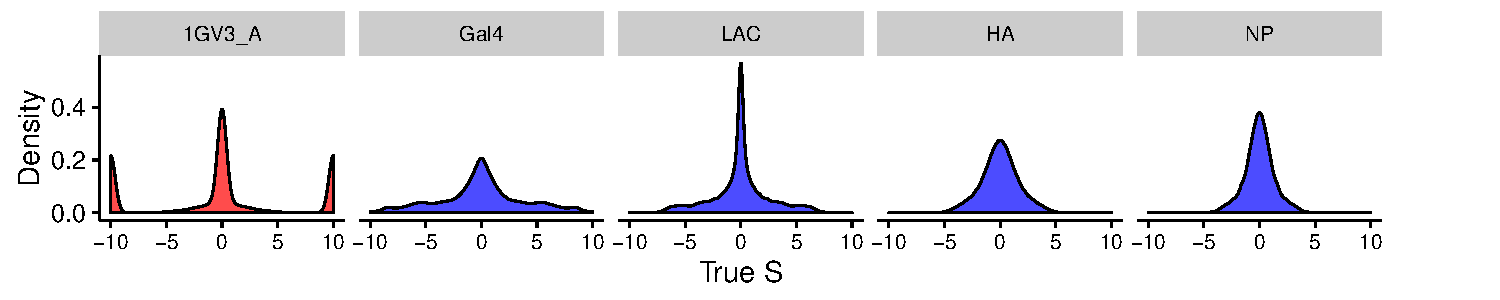
\includegraphics[width=6in]{Figures/small_selcoeffs.pdf}}
  \caption{\label{fig:example-selcoeffs} Distributions of true scaled selection coefficients, $S$, for a representative natural simulation (1GV3\_A) and each DMS simulation. Scaled selection coefficients have been binned at $S\geq10$ and $S\leq-10$ for visualization. Histograms depicting the true $S$ distribution for all other natural simulations are provided in Figures S8--S10. $S$ distributions shown represent the selection coefficients among all possible single-nucleotide changes, across all sites.}
\end{figure}



\vspace{3cm}
\begin{figure}[htbp]
  \centerline{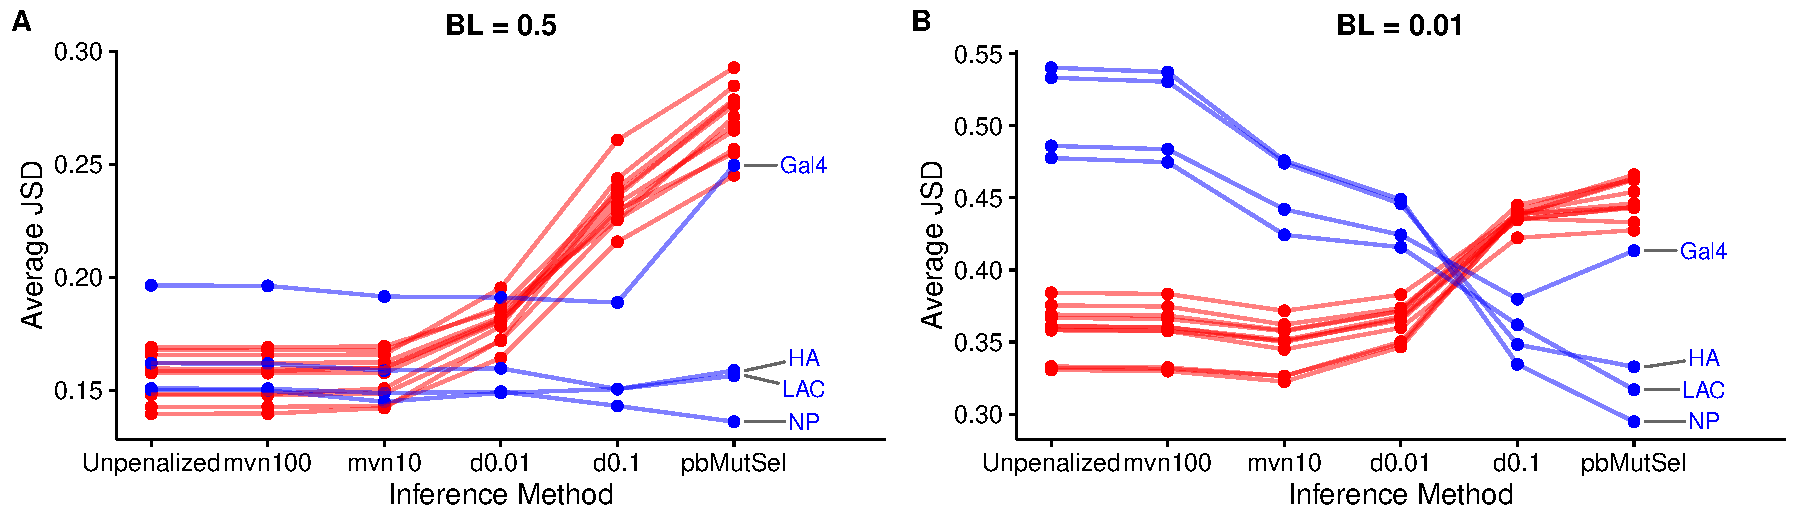
\includegraphics[width=5in]{Figures/jsd_lineplot.pdf}}
  \caption{\label{fig:jsd_lineplots} Jensen-Shannon distance between true and inferred amino-acid frequency distributions. (A) BL=0.5 simulations. (B) BL=0.01 simulations. Each point represents the mean JSD across sites for a given simulation, and labeled points correspond to DMS simulations. Note that the y-axis of each panel has a different range.}
\end{figure}



\vspace{3cm}
\begin{figure}[htbp]
  \centerline{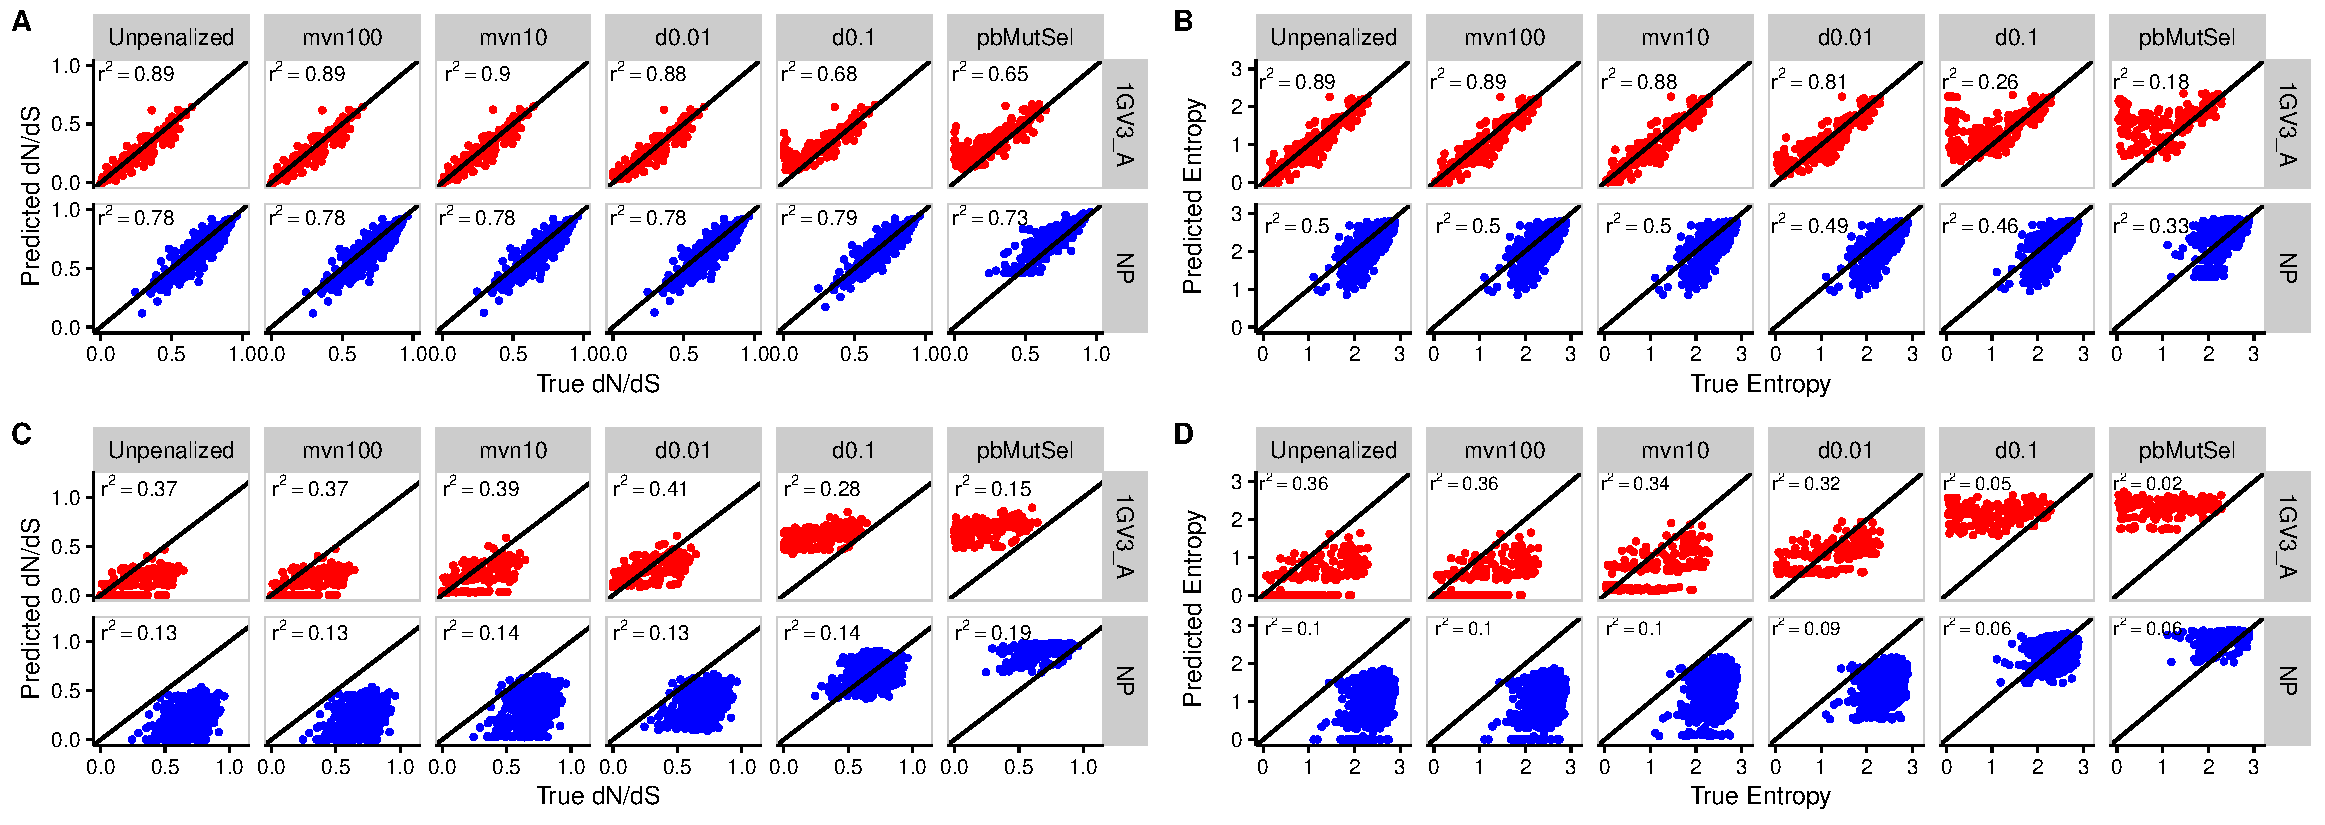
\includegraphics[width=7.5in]{Figures/scatter_dnds_entropy_full.pdf}}
\caption{\label{fig:scatter}
Performance of mutation--selection model inference platforms for one representative natural (1GV3\_A) and DMS (NP) simulation each. (A) $dN/dS$ predicted from model inference vs. true $dN/dS$, under branch lengths of 0.5. (B) Entropy calculated from model inferences vs. true entropy, under branch lengths of 0.5. (C) $dN/dS$ predicted from model inference vs. true $dN/dS$, under branch lengths of 0.01. (D) Entropy calculated from model inferences vs. true entropy, under branch lengths of 0.01. In each panel, the straight line indicates the $y=x$ line. Scatterplots for all simulated datasets are provided in Figures S3--S6.}
\end{figure}


\vspace{3cm}
\begin{figure}[htbp]
  \centerline{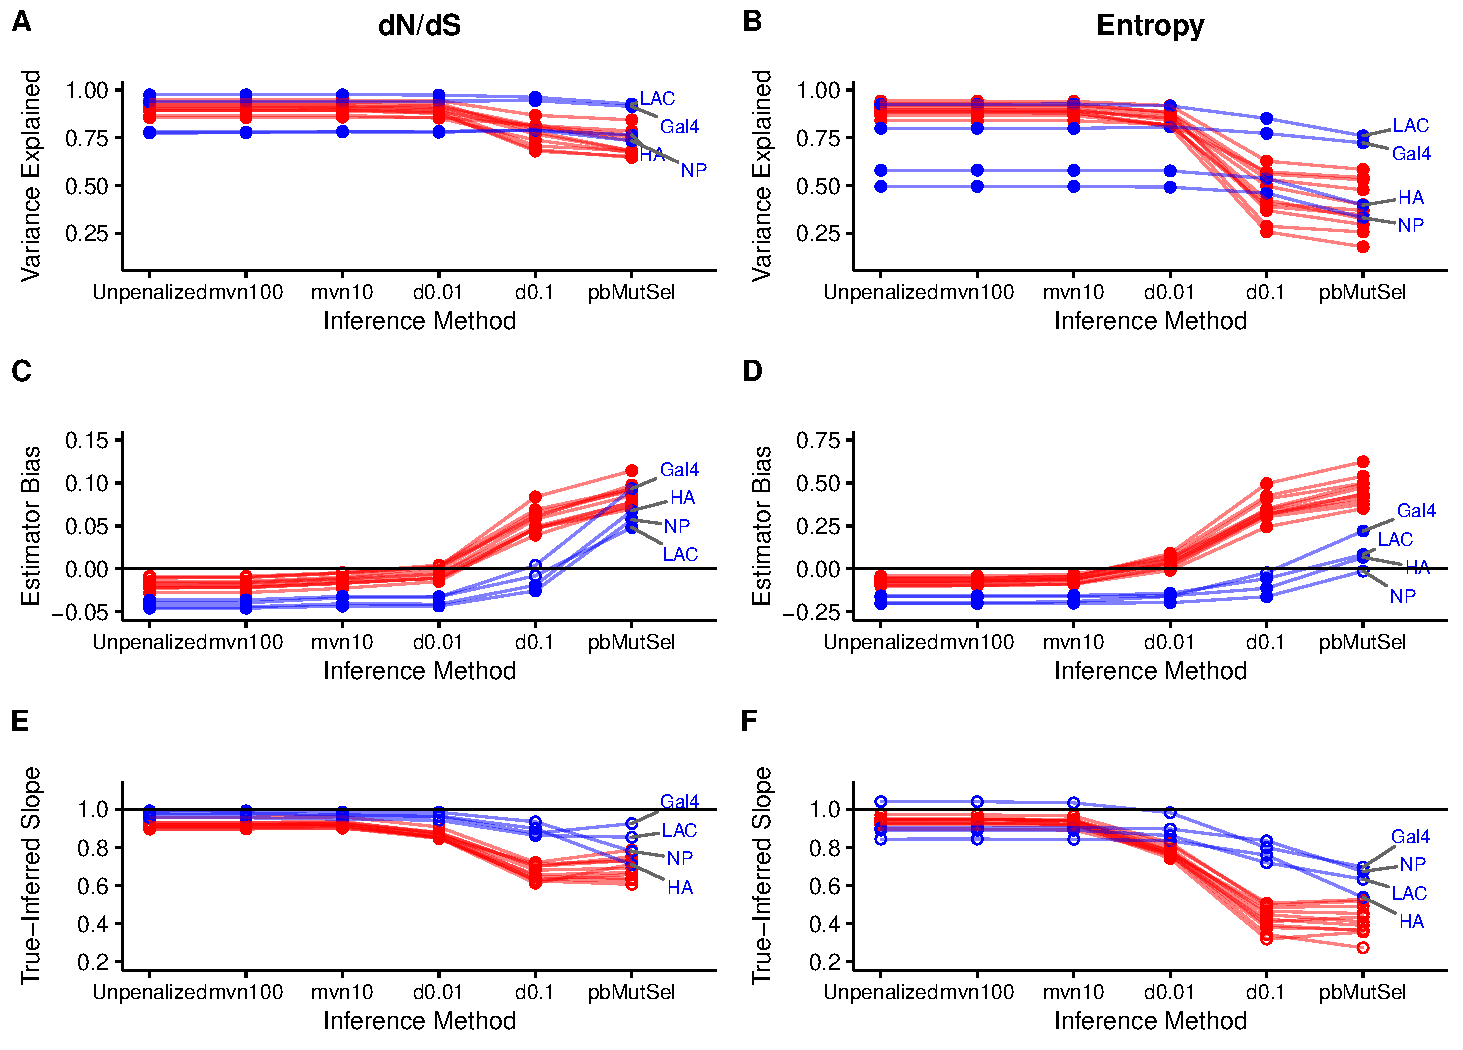
\includegraphics[width=5.5in]{Figures/r2_bias_slope_bl0_5.pdf}}
\caption{\label{fig:r2_bias_slope}
Performance of mutation--selection model inference platforms for branch lengths of 0.5. Labeled points correspond to DMS simulations. (A-B) $r^2$ between true and inferred $dN/dS$ (A) and entropy (B) across inference methods, for all simulated datasets. (C-D) Estimator bias of inference methods relative to true $dN/dS$ (C) and entropy (D) values, for all simulated datasets. Open points indicate biases that were not significantly different from 0 (Bonferroni-corrected $P>0.05$, test for intercept in linear model), and solid points indicate biases that were significantly different from 0 (Bonferroni-corrected $P<0.05$). The straight line indicates an estimator bias of 0, meaning an unbiased predictor. Note that panels (C-D) use different y-axis ranges, due to the different scales between $dN/dS$ and entropy. (E-F) Slope for the linear relationship of inferred regressed on true $dN/dS$ (E) and entropy (F) values. Open points indicate slopes that were not significantly different from 1 (Bonferroni-corrected $P>0.05$, test for slope in linear model not equal to 1), and solid points indicate biases that were significantly different from 1 (Bonferroni-corrected $P<0.05$). The straight line indicates the null slope of 1. A corresponding figure for simulations using branch lengths of 0.01 is in Figure S7.}
\end{figure}



\vspace{3cm}
\begin{figure}[htbp]
  \centerline{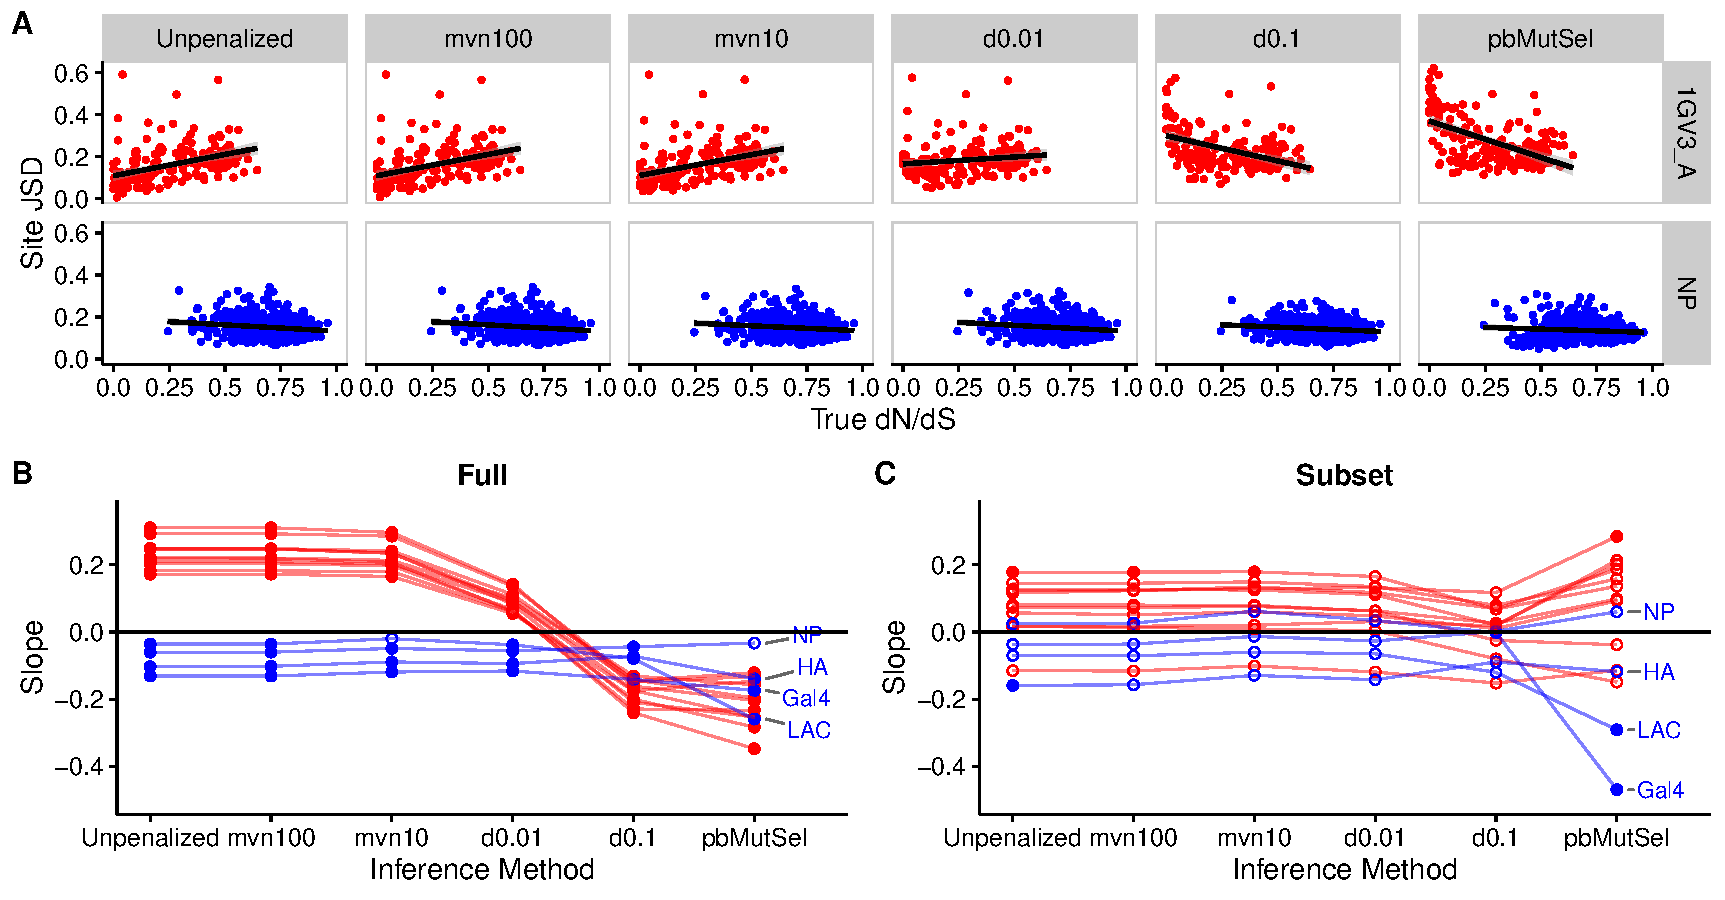
\includegraphics[width=7in]{Figures/jsd_truednds_slopes.pdf}}
  \caption{\label{fig:jsd_vs_dnds} The site-specific Jensen-Shannon distance between true and inferred amino-acid frequencies depends both on selective constraint and inference method. Results are shown for simulations with branch lengths of 0.5. Labeled points correspond to DMS simulations. (A) Site JSD regressed on true site $dN/dS$. The line in each panel indicates the linear regression line. (B) Slope of relationship shown in panel (A) for all simulated datasets. (C) Slope of relationship shown in panel (A) for all simulated datasets, considering only a subset of sites whose true $dN/dS$ falls in the range $dN/dS\in[0.3,0.6]$. For panels (B) and (C), the straight line indicates the $y=0$ line, meaning no linear relationship between JSD and $dN/dS$. Open points indicate slopes that were not significantly different from 0 (Bonferroni-corrected $P>0.05$), and solid points indicate slopes that were significantly different from 0 (Bonferroni-corrected $P<0.05$).}
 \end{figure}


\vspace{3cm}
\begin{figure}[htbp]
  \centerline{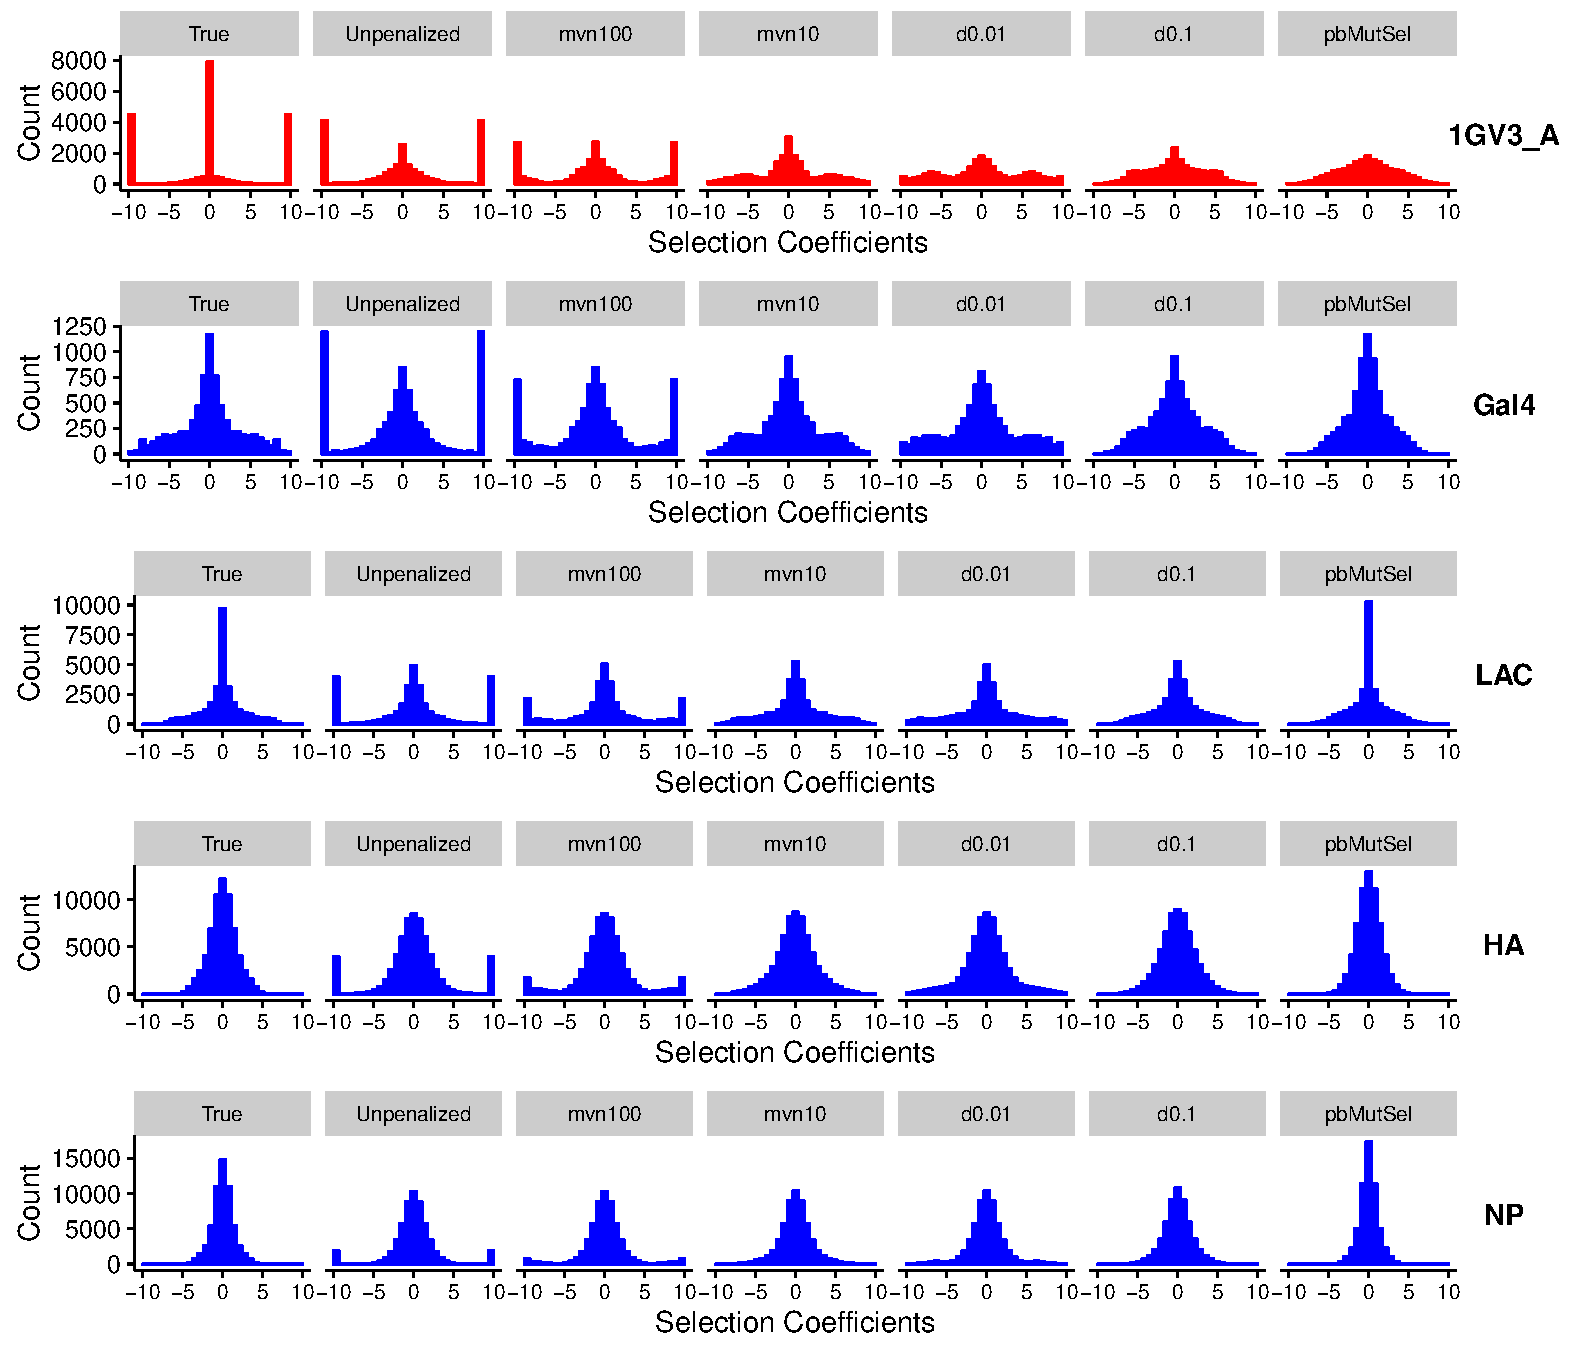
\includegraphics[width=6in]{Figures/selcoeff_histograms_subset.pdf}}
  \caption{\label{fig:selcoeffs_histograms} True and inferred distributions of scaled selection coefficients for a subset of simulations, under branch lengths of 0.5. Histograms for simulations not shown here are in Figures S8-10. $S$ distributions shown represent the selection coefficients among all possible single-nucleotide changes, across all sites.}
\end{figure}


\end{document}
